\documentclass[UTF8]{beamer}
\usepackage{ctex}
\usepackage{graphicx}
\usepackage{amsmath}
\usepackage{setspace}
\usepackage{float} 
\usepackage{multirow}
\usepackage{array}
\usepackage{enumerate}
\usepackage{booktabs}
\usepackage{indentfirst} 
\usepackage[style=mla]{biblatex}
\usepackage{subfigure}
\usepackage{hyperref}
\usepackage{ulem}
\usepackage{textpos}

\definecolor{Turquoise3}{RGB}{0, 134, 139}
\renewcommand{\emph}[1]{{\color{Turquoise3}\textsl{#1}}}
 \newcommand{\F}{\mathbb{F}} \newcommand{\R}{\mathbb{R}} \newcommand{\Q}{\mathbb{Q}}
\newcommand{\N}{\mathbb{N}}
\newcommand{\myseries}[2]{$#1_1,#1_2,\dots,#1_#2$}
\newcommand{\nullspace}{~\\[15pt]}

\usetheme{Madrid}
\setbeamertemplate{navigation symbols}{}

\addtobeamertemplate{frametitle}{}{
\begin{textblock*}{100mm}(0.85\textwidth,-1cm)

\includegraphics[height=1cm]{logo.png}
\end{textblock*}}

\definecolor{themecolor}{RGB}{25,25,112} 

\usecolortheme[named=themecolor]{structure}

\setbeamertemplate{items}[default]


\title{Some Tips for \textbf{VV285}}
\subtitle{"Learn Well and Have Fun"}
\institute[UM-SJTU JI]{Univerity of Michigan-Shanghai Jiao Tong University Joint Institute}
\author{Zhang Xingjian}

\begin{document}

\begin{frame}
    \titlepage
    \begin{center}
        
\includegraphics[height=2cm]{logo2.png}
    \end{center}
\end{frame}

\begin{frame}
    \frametitle{Course Description}
    The course revolves around three themes:
    \begin{enumerate}
        \item \textbf{Linear Algebra}\\
              finite dimensional vector spaces, linear maps, matrices and determinants...
        \item \textbf{Differential Calculus}\\
              derivatives, curves, potential functions and extrema...
        \item \textbf{Vector Fields \& Integral Calculus}\\
              line integrals, surface integral, circulation, flux, integrations in practice...
    \end{enumerate}
    \begin{figure}[H]
    \centering
    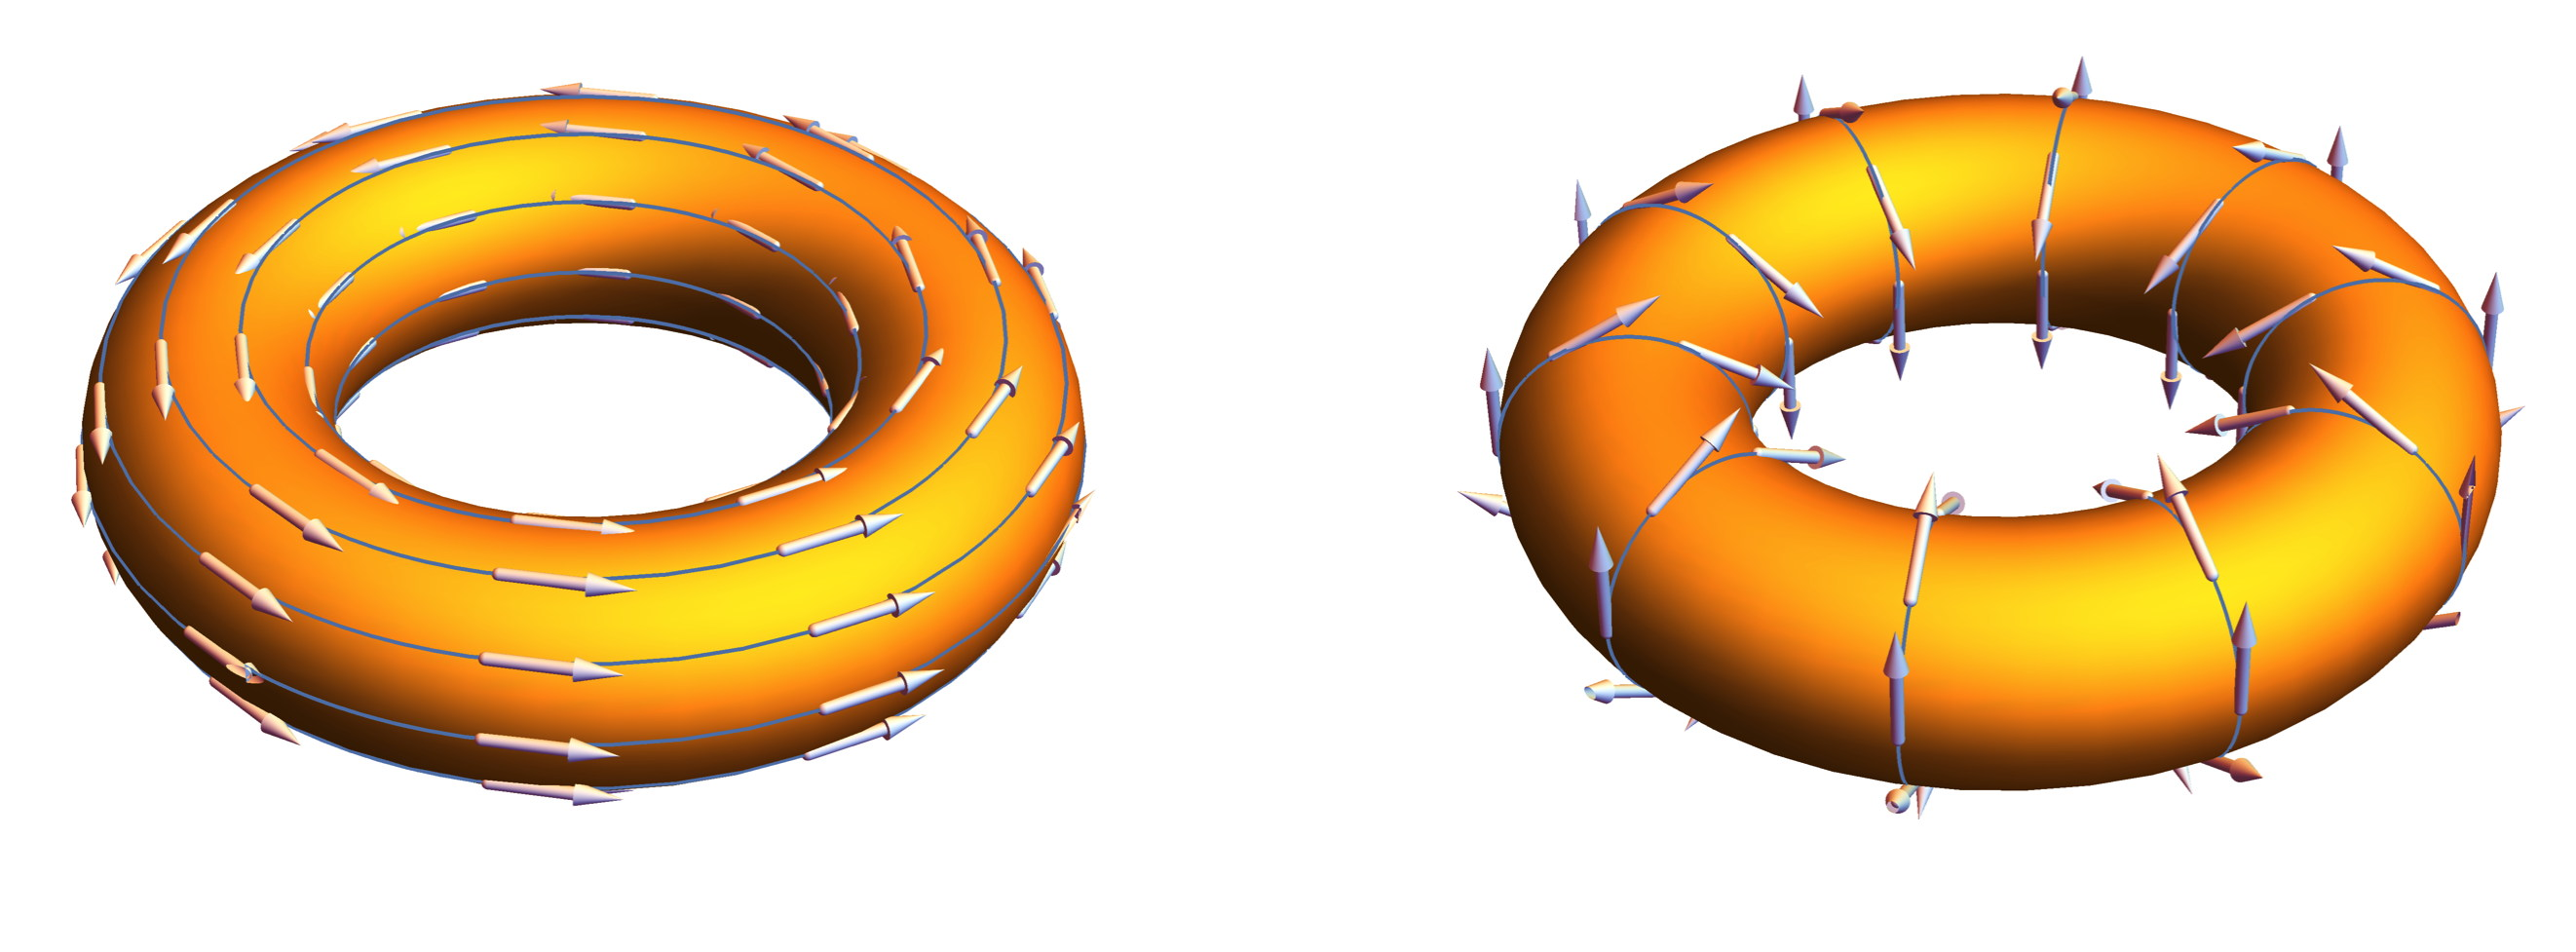
\includegraphics[width=0.8\textwidth]{2020-05-05-17-54-53.png}
    \caption{Vector Field}
    \end{figure}
    
\end{frame}

\begin{frame}
    \frametitle{Grading}
    \begin{table}[ht]
        \begin{tabular}{cc}
            \hline
            Component    & Proportion \\ \hline
            Mid 1        & 30\%       \\
            Mid 2        & 30\%       \\
            Final        & 30\%       \\
            Term Project & 10\%       \\ \hline
        \end{tabular}
    \end{table}
    Generally, 3 Q3 $\rightarrow$ A+, 3 Q2 $\rightarrow$ B+.
\end{frame}

\begin{frame}
    \frametitle{VV186 vs. VV285}
    VV285 is
    \begin{enumerate}
        \item more general,     e.g. $\R\Rightarrow\R^n, \dfrac{d}{dx}\Rightarrow\dfrac{\partial}{\partial x}$
        \item more concrete (especially in calculus),
        \item more interesting (it depends on you!),
        \item \sout{relatively easier (in exams)},
        \item more practical (in homeworks/project).
    \end{enumerate}
    \nullspace
    There is connection between VV285 and VV186, but the connection is not that strong. Therefore,\\
    - Don't panic if you didn't do well in VV186.\\
    - Don't be over-confident if you did a great job in VV186.
\end{frame}

\begin{frame}
    \frametitle{Assignments \& Project}
    For assignment:
    \begin{enumerate}
        \item Similar with VV186.
        \item Exams may contain concepts that appeared in your assignments.
        \item Readability is important. (Words speak louder than math symbols.)
    \end{enumerate}

    For project:
    \begin{enumerate}
        \item Randomly assigned teams.
        \item Differ from an assignment in format, content and language.
        \item Start early or stay up late.
    \end{enumerate}
\end{frame}

\begin{frame}
    \frametitle{Recitation Class}
    In RC, 4 parts will be covered:
    \begin{enumerate}
        \item Recap of the lecture content
        \item Exercises (often basic)
        \item Review of assignment problems
        \item Extension of the lecture content
    \end{enumerate}
    \nullspace
    Language: English
\end{frame}

\begin{frame}
    \frametitle{Reference Books}
    \begin{enumerate}
        \item Generally, you can get a good grade without recourse to any reference textbooks.
        \item However, if needed, a list of recommended textbooks can be found in \textit{vv285 Course Description}.
        \item Chinese textbooks are not recommended.
    \end{enumerate}
\end{frame}

\begin{frame}
    \frametitle{Some tips}
    \begin{itemize}
        \item
              For assignment,
              \begin{itemize}
                  \item think carefully,
                  \item do it on your own,
                  \item catch the key point (pay attention to any new concept in your assignment).
              \end{itemize}
        \item During the class, focus on \textbf{the general ideas, the connections between new \& old knowledge and the remarks/discussions}. Do not panic if you cannot understand some details during the lecture. (不求甚解) Just leave them to your own time after class, and push yourself to figure them out. \textbf{To review the lecture slides is indispensible if you want to obtain a deep understanding of VV285.}
    \end{itemize}
\end{frame}

\begin{frame}
    \frametitle{Some tips}
    \begin{itemize}
        \item Discuss with your friends to discover new perspectives.
        \item You are encouraged to come to RC \& OH. Active \textbf{feedback} is important in online RC.
    \end{itemize}
\end{frame}

\begin{frame}
    \frametitle{End}
    \begin{center}
        \huge
        Learn Well\\
        And\\
        Have Fun!\\
        \nullspace
        \large
        Q\&A
    \end{center}
\end{frame}

\end{document}